\chapter*{Anhang}
\addcontentsline{toc}{chapter}{Anhang}
\section*{Anhangverzeichnis}
\vspace{-8em}

% vor \listofanhang müssen Einrückungen angepasst werden
\abstaendeanhangverzeichnis

\listofanhang
\clearpage
\spezialkopfzeile{Anhang} % damit in der Kopfzeile das Wort "Anhang" angezeigt wird

\anhang{Projektrollen und Verantwortlichkeiten}\label{anhang:kap1}
% \anhangteil{Unterkapitel 1}\label{anhang:ukap1}
\begin{figure}[H]
  \centering
  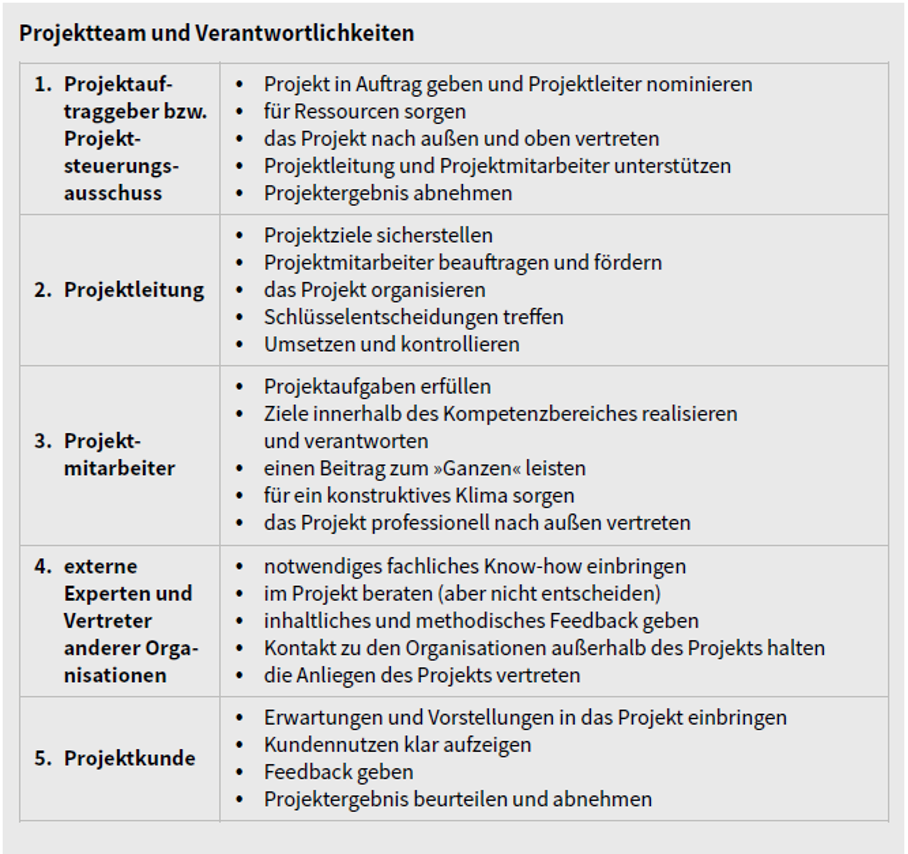
\includegraphics[width=0.8\linewidth]{graphics/pr_ve.png}
  \caption[Rollen und Verantwortlichkeiten in Projekten.]{Rollen und Verantwortlichkeiten in Projekten.\protect\footnotemark}\label{abb:pr_ve}
\end{figure}
\footnotetext{\cite[Enthalten in:][90]{stoegerWirksamesProjektmanagementMit2019}}
\anhang{Discord-Server Organisationsstruktur}\label{anhang:kap2}

\lstset{language=TeX, % hervorzuhebende Keywords definieren
  morekeywords={anhang, anhangteil}
}